\documentclass[tikz]{standalone}
\usepackage{tikz}
\usepackage{../../../../glossary}
\usetikzlibrary{arrows.meta, chains, positioning}

% arara: pdflatex
% arara: latexmk: { clean: partial }
\begin{document}
    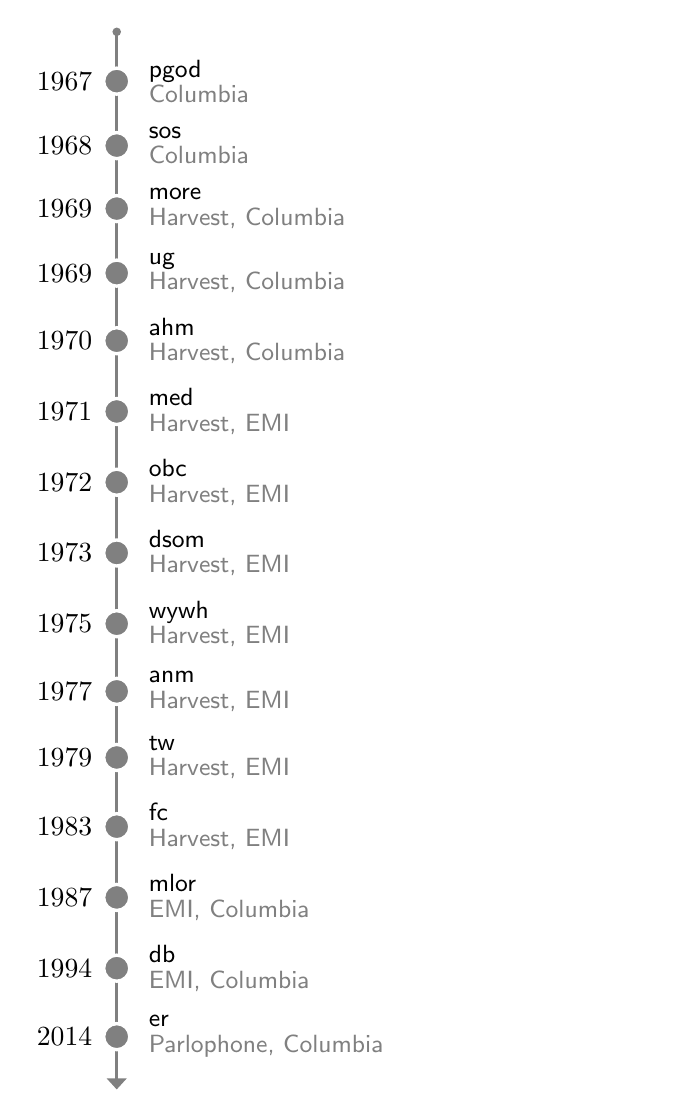
\begin{tikzpicture}[
        node distance = 1mm and 3mm,
        start chain = A going below,
        dot/.style = {circle, draw=white, very thick, fill=gray,
                        minimum size=3mm},
        box/.style = {rectangle, text width=62mm,
                        inner xsep=4mm, inner ysep=1mm,
                        font=\sffamily\small\linespread{0.84}\selectfont,
                        on chain},
                                ]
        \begin{scope}[every node/.append style={box}]
            \node { 
                \acrlong{pgod}   \\      % A-1
                \textcolor{gray}{Columbia}     \\
                % Universidad Antonio de Nebrija, Madrid
            } ;
            \node { 
                \acrlong{sos}   \\
                \textcolor{gray}{Columbia}     \\
                % Universidad Antonio de Nebrija, Madrid
            } ;
            \node { 
                \acrlong{more}   \\      % A-3
                \textcolor{gray}{Harvest, Columbia}     \\
                % Universidad Antonio de Nebrija, Madrid
            } ;
            \node { 
                \acrlong{ug}   \\      % A-1
                \textcolor{gray}{Harvest, Columbia}     \\
                % Universidad Antonio de Nebrija, Madrid
            } ;
            \node { 
                \acrlong{ahm}   \\
                \textcolor{gray}{Harvest, Columbia}     \\
                % Universidad Antonio de Nebrija, Madrid
            } ;
            \node { 
                \acrlong{med}   \\      % A-3
                \textcolor{gray}{Harvest, EMI}     \\
                % Universidad Antonio de Nebrija, Madrid
            } ;
            \node { 
                \acrlong{obc}   \\      % A-3
                \textcolor{gray}{Harvest, EMI}     \\
                % Universidad Antonio de Nebrija, Madrid
            } ;
            \node { 
                \acrlong{dsom}   \\      % A-3
                \textcolor{gray}{Harvest, EMI}     \\
                % Universidad Antonio de Nebrija, Madrid
            } ;
            \node { 
                \acrlong{wywh}   \\      % A-3
                \textcolor{gray}{Harvest, EMI}     \\
                % Universidad Antonio de Nebrija, Madrid
            } ;
            \node { 
                \acrlong{anm}   \\      % A-3
                \textcolor{gray}{Harvest, EMI}     \\
                % Universidad Antonio de Nebrija, Madrid
            } ;
            \node { 
                \acrlong{tw}   \\      % A-3
                \textcolor{gray}{Harvest, EMI}     \\
                % Universidad Antonio de Nebrija, Madrid
            } ;
            \node { 
                \acrlong{fc}   \\      % A-3
                \textcolor{gray}{Harvest, EMI}     \\
                % Universidad Antonio de Nebrija, Madrid
            } ;
            \node { 
                \acrlong{mlor}   \\      % A-3
                \textcolor{gray}{EMI, Columbia}     \\
                % Universidad Antonio de Nebrija, Madrid
            } ;
            \node { 
                \acrlong{db}   \\      % A-3
                \textcolor{gray}{EMI, Columbia}     \\
                % Universidad Antonio de Nebrija, Madrid
            } ;
            \node { 
                \acrlong{er}   \\      % A-3
                \textcolor{gray}{Parlophone, Columbia}     \\
                % Universidad Antonio de Nebrija, Madrid
            } ;
        \end{scope}
        \draw[very thick, gray, {Circle[length=3pt]}-{Triangle[length=4pt)]},
            shorten <=-3mm, shorten >=-3mm]           % <--- here is adjusted additional arrow's 
            (A-1.north west) -- (A-15.south west);
        \foreach \i [ count=\j] in {
                1967, 
                1968, 
                1969,
                1969, 
                1970, 
                1971,
                1972,
                1973,
                1975,
                1977,
                1979,
                1983,
                1987,
                1994,
                2014
            }
            \node[dot,label=left:\i] at (A-\j.west) {};
    \end{tikzpicture}
\end{document}